\documentclass[tikz,border=2pt]{standalone}
\usepackage{graphicx}
\usepackage{xcolor}
\usepackage{array}
\usepackage{colortbl}
\usepackage{tabularx}
\usepackage[scaled=0.93]{helvet}
\renewcommand{\familydefault}{\sfdefault}

\definecolor{UTBurnt}{RGB}{191,87,0}
\definecolor{UTDark}{RGB}{51,63,72}
\definecolor{UTLight}{RGB}{248,246,242}

\newcommand{\metricrow}[2]{#1 & \textbf{\color{UTBurnt}#2}\\}
\setlength{\tabcolsep}{4pt}
\renewcommand{\arraystretch}{1.12}

\begin{document}
\begin{tikzpicture}
  \node[anchor=north west,inner sep=0pt] at (0,0)
    {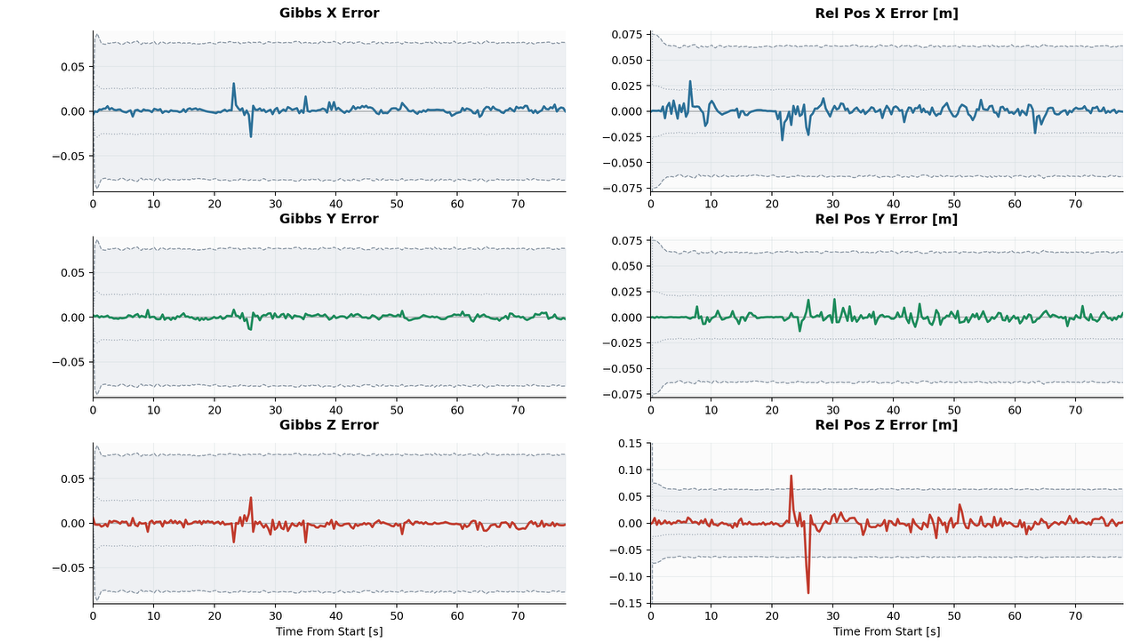
\includegraphics[width=12.8cm]{fig_filter_error_panel.png}};

  \node[anchor=north west,text width=12.8cm,inner sep=0pt] at (0,-7.42) {
    \scriptsize
    \begin{tabularx}{12.8cm}{>{\raggedright\arraybackslash}X >{\raggedleft\arraybackslash}p{2.8cm}}
      \rowcolor{UTBurnt}\color{white}\bfseries Performance average & \color{white}\bfseries Value\\
      \rowcolor{UTLight}\metricrow{Translation, in-plane Root Mean Square Error (RMSE)}{0.48 cm}
      \metricrow{Translation, depth RMSE}{1.68 cm}
      \rowcolor{UTLight}\metricrow{Euler rotation RMSE}{1.05 deg}
      \metricrow{Measurement frequency}{2.85 Hz}
    \end{tabularx}
  };

\end{tikzpicture}
\end{document}
